\section{Proposed Model}
In this section, we first define our approach to generate knowledge graph from document text and graph translation before generating graph embedding for CapsNet.
\subsection{Knowledge Graph from Text}
To build knowledge graph from document text requires extract entities and relations. This approach is ideal for fixed domain such as social networks and HIN from social networks. When domain is not fixed, for large number of documents, it becomes impractical to gather such training data that can do entity extraction. As defined earlier, we are creating multi dimensional HIN that is higher level abstraction of domain and relationship between nodes. Hence, we use pre-trained model BERT\cite{devlin2018bert}.

BERT model comes pre-trained on large corpus.  

\subsection{Graph Translation}
Our goal is to derive $ S= \{ s_i_j \}$ that is similarity matrix of directed graph $ G $, where  $ s_i_j (i, j=1, 2, ... n) $ is the similarity score between node $i$ and $j$. $G=(E,V,W)$ where $V=\{ v_1,...,_n \} $ is the set of vertices and  $E  \subseteq V \times V$ set of edges. Let $ n $ be the number of vertices and $ m $ the number of edges. $G$ is directed graph with $e_i_j=1$ for edge $i \to j$ and $e_i_j=-1$ for edge $j \to i$. We allow, each edge $(i,j)$ to have corresponding weight $w_i_j \in W$. Furthermore, each vertex $v_i$ has feature vector $l_i$.
CapsGraph has three steps: 1. Generate static sub-graphs with defined vertex ordering, 2. Create convolution layers using local substructure, 3. Learn graph structures using capsule filters.

\subsection{Capsule Network for Graph}

\begin{figure}[!htbp]
  \centering
  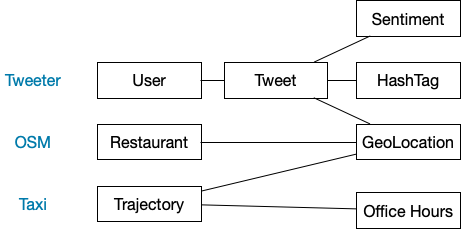
\includegraphics[width=\linewidth,height=\textheight,keepaspectratio]{images/Sample_Data}
  \caption{Original Dataset}
  \label{sample_data}
\end{figure}

\subsection{Graph Translation Algorithm}
In order to create neighbourhood matrix that represents vertex in consistent order we used sorting algorithm based on in-degree and out-degree of nodes. First, part is to create sub-graph that is represents context of node entities. In order to generate sub-graph, we first visit each neighboring node and compare depth from starting node to connected edges of visiting node which becomes terminating factor for sub-graph.

% \subsection{Graph Convolutional Layer}
% \subsection{Capsule Layer}
% \begin{figure}
% \begin{tikzpicture}[scale=1.8, auto,swap]
%     % Draw a 7,11 network
%     % First we draw the vertices
%     \foreach \pos/\name in {{(0,2)/a}, {(2,1)/b}, {(4,1)/c},
%                             {(0,0)/d}, {(3,0)/e}, {(2,-1)/f}, {(4,-1)/g}}
%         \node[vertex] (\name) at \pos {$\name$};
%     % Connect vertices with edges and draw weights
%     \foreach \source/ \dest /\weight in {b/a/7, c/b/8,d/a/5,d/b/9,
%                                          e/b/7, e/c/5,e/d/15,
%                                          f/d/6,f/e/8,
%                                          g/e/9,g/f/11}
%         \path[edge] (\source) -- node[weight] {$\weight$} (\dest);
%     % Start animating the vertex and edge selection. 
%     \foreach \vertex / \fr in {d/1,a/2,f/3,b/4,e/5,c/6,g/7}
%         \path<\fr-> node[selected vertex] at (\vertex) {$\vertex$};
%     % For convenience we use a background layer to highlight edges
%     % This way we don't have to worry about the highlighting covering
%     % weight labels. 
%     \begin{pgfonlayer}{background}
%         \pause
%         \foreach \source / \dest in {d/a,d/f,a/b,b/e,e/c,e/g}
%             \path<+->[selected edge] (\source.center) -- (\dest.center);
%         \foreach \source / \dest / \fr in {d/b/4,d/e/5,e/f/5,b/c/6,f/g/7}
%             \path<\fr->[ignored edge] (\source.center) -- (\dest.center);
%     \end{pgfonlayer}
% \end{tikzpicture}
% \end{figure}

\FloatBarrier
% \subsection{Training}

\begin{figure}[!htbp]
  \centering
  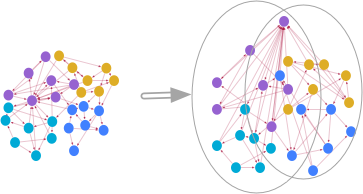
\includegraphics[width=\linewidth,height=\textheight,keepaspectratio]{images/graph_normalization}
  \caption{Graph Representation Model}
  \label{graph_model}
\end{figure}